\chapter{Physics: Quantum Field Theories}

The Standard Model (SM) of particle physics classifies all known
{\it elementary particles}, i.e. particles with no known substructure,
and describes three fundamental forces: the electromagnetic,
weak, and strong forces. Elementary particles can be divided into
{\it matter particles} (quarks and leptons); {\it gauge bosons}, which mediate
the three aforementioned forces; and a {\it scalar boson}, the Higgs boson,
whose field interacts directly with elementary particles that thereby
acquire their mass. For each particle there exists a corresponding
antiparticle; sometimes a particle is its own antiparticle.
Figure~\ref{fig:SM} gives a schematic overview of the SM.
The SM has a long history of experimental confirmations culminating
in the 2012 discovery of the Higgs boson by the ATLAS and CMS
experiments~\cite{aad_observation_2012,chatrchyan_observation_2012}.

\begin{figure}
  \centering
  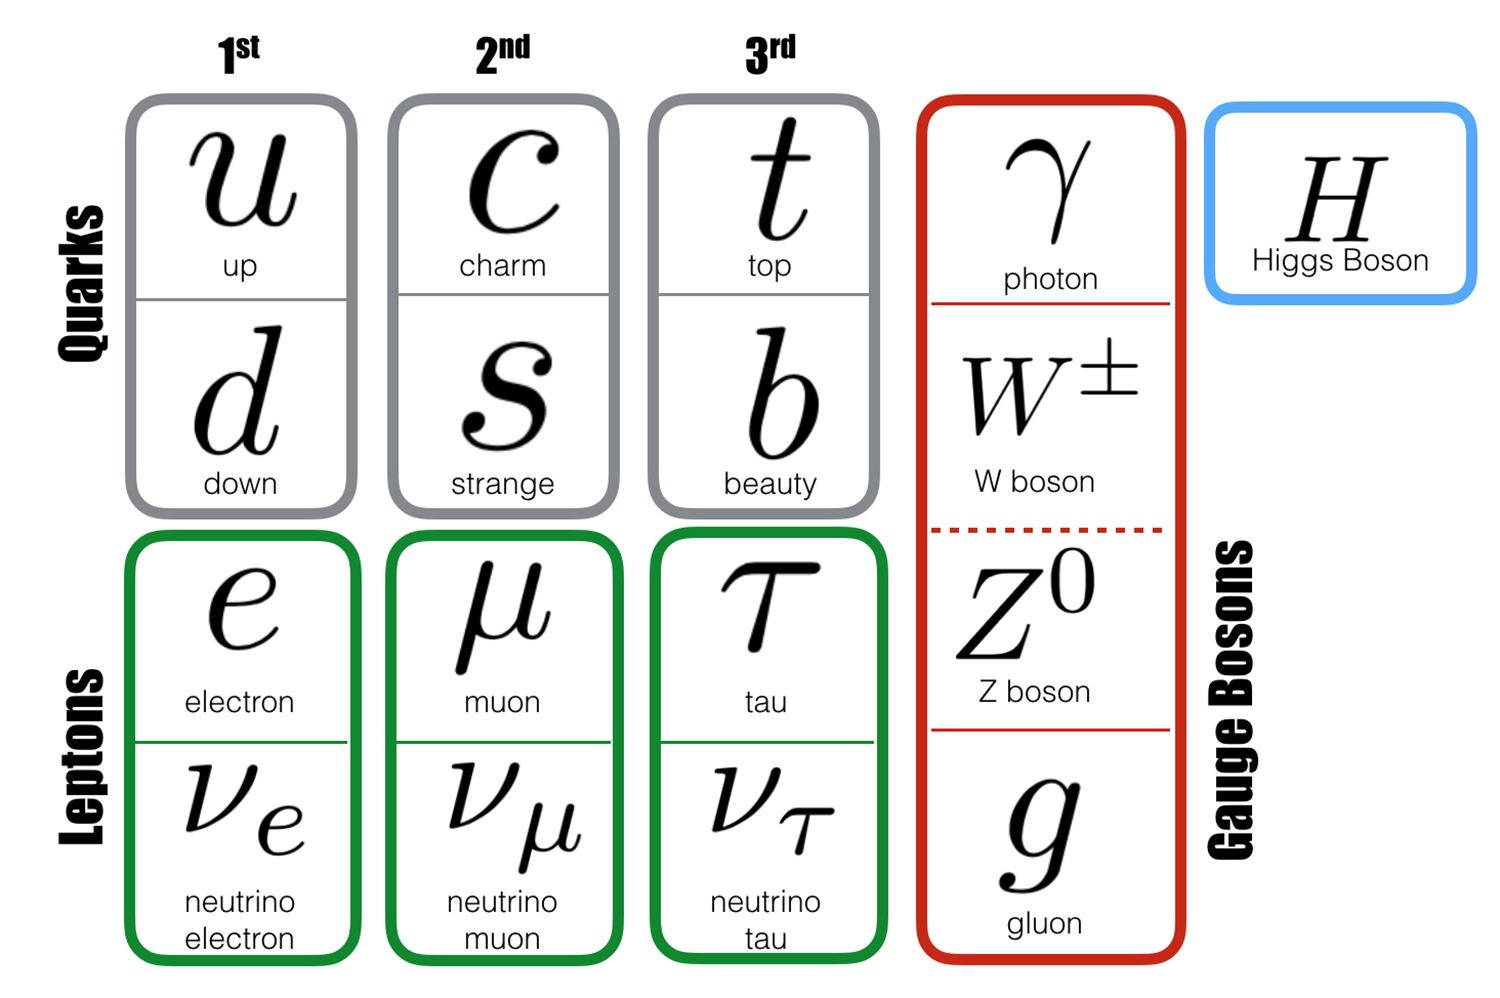
\includegraphics[width=0.95\linewidth]{figs/SM.png}
  \caption{Summary of elementary SM particles. The first three columns give
           the three generations of matter particles. Image taken
           from the Physics Institute at University of 
           Zurich~\cite{zurich_SM}.}
  \label{fig:SM}
\end{figure}

The theoretical framework underlying the SM is an example of a Quantum 
Field Theory (QFT). QFTs are consistent with both quantum mechanics and
relativity. Lattice gauge theories are a kind of QFT; therefore it is
important for the reader to know a little bit about them.

\section{The principle of stationary action}

This section follows a fairly well known and delightful lecture by Feynman
\cite{caltech}.

\section{The non-relativistic and classical limits}

In this section I briefly give some intuition for how mundane Newtonian
physics can be recovered from the more esoteric relativistic and quantum
theories. Namely I want to focus on the following two phrases:
\begin{enumerate}
  \item The non-relativistic limit is $c\to\infty$.
  \item The classical limit is $\hbar\to0$.
\end{enumerate}
I don't think I have the understanding to prove anything, but at least I
can provide some ideas and examples that can make you believe these
two statements.

The non-relativistic limit is, I think, the easier to understand. When we
learn about relativity, the speed of light $c$ is taken as a ``cosmic speed
limit"; correspondingly, sending $c\to\infty$ lifts the speed limit, and
so perhaps it's not surprising that Galilean physics is recovered.
More explicitly, we can see what happens to the Lorentz factor $\gamma$ and
Einstein velocity addition formula under these limits. For the former
we find
\begin{equation}
  \lim_{c\to\infty}\gamma
  =\lim_{c\to\infty}\frac{1}{\sqrt{1-v^2/c^2}}=1,
\end{equation}
i.e. there is no longer any time dilation or length contraction.
Meanwhile when $c\gg v$, we find for the velocity addition formula 
\begin{equation}
  v_1\oplus v_2
  =\frac{v_1/c + v_2/c}{1+v_1v_2/c^2}
  \approx \frac{v_1}{c} + \frac{v_2}{c}, 
\end{equation}
i.e. it reduces to Galilean velocity addition.

For the classical limit, one can look at specific, simple examples, such as
the quantum harmonic oscillator. In QM, the energy levels of this system
are given by
\begin{equation}
  E_n=\hbar\omega\left(n+\frac{1}{2}\right).
\end{equation}
In the $\hbar\to0$ limit, one therefore sees that the differences in energy
become continuous rather than discrete. More generally one can look at
the Heisenberg uncertainty relation,
\begin{equation}
  \Delta p\Delta x\geq \frac{\hbar}{2},
\end{equation}
and when $\hbar=0$, you are once again allowed to know position and
momentum simultaneously.

\section{The path integral}

\bibliographystyle{unsrtnat}
\bibliography{bibliography}
